\documentclass[border=10pt]{standalone}
\usepackage{tikz}\usepackage{amsmath}\usetikzlibrary{arrows.meta}
\definecolor{cine}{HTML}{2e4824}\definecolor{cpre}{HTML}{1a4a7a}\definecolor{cvis}{HTML}{b07828}\definecolor{cgra}{HTML}{6a3e18}
\begin{document}
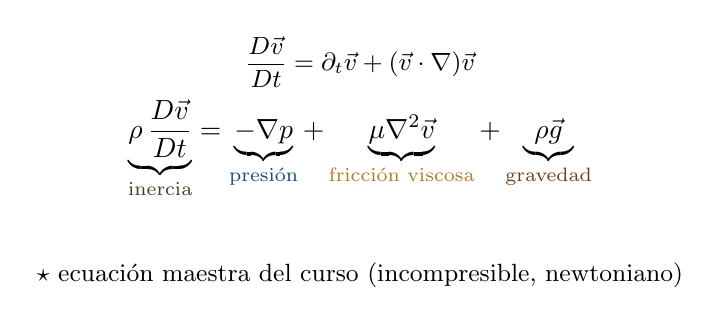
\begin{tikzpicture}[line width=0.9pt]
  \node at (0,0.7){\small $\dfrac{D\vec v}{Dt}=\partial_t\vec v+(\vec v\cdot\nabla)\vec v$};
  \node at (0,-0.4){$\displaystyle \underbrace{\rho\,\frac{D\vec v}{Dt}}_{\textcolor{cine}{\text{inercia}}}=\underbrace{-\nabla p}_{\textcolor{cpre}{\text{presión}}}+\underbrace{\mu\nabla^2\vec v}_{\textcolor{cvis}{\text{fricción viscosa}}}+\underbrace{\rho\vec g}_{\textcolor{cgra}{\text{gravedad}}}$};
  \node at (0,-2.0){\small $\star$ ecuación maestra del curso (incompresible, newtoniano)};
\end{tikzpicture}
\end{document}
